\documentclass{beamer}
%
% Choose how your presentation looks.
%
% For more themes, color themes and font themes, see:
% http://deic.uab.es/~iblanes/beamer_gallery/index_by_theme.html
%
\mode<presentation>
{
  \usetheme{Warsaw}      % or try Darmstadt, Madrid, Warsaw, ...
  \usecolortheme{default} % or try albatross, beaver, crane, ...
  \usefonttheme{default}  % or try serif, structurebold, ...
  \setbeamertemplate{navigation symbols}{}
  \setbeamertemplate{caption}[numbered]
} 

\usepackage[english]{babel}
\usepackage[utf8x]{inputenc}
\usepackage{graphicx}
\usepackage[ELEC]{aaltologo}

\title[SSL X.509 commonName Attack]{SSL X.509 commonName $\backslash0$ Prefix Attack}
\author{Riku Lääkkölä \and Tero Marttila \and Tero Paloheimo}
\institute{Aalto ELEC}
\date{11.2.2014}
\logo{\AaltoLogoRandomSmall{0.3}}

\begin{document}

\begin{frame}
  	\titlepage
\end{frame}

% Uncomment these lines for an automatically generated outline.
%\begin{frame}{Outline}
%  \tableofcontents
%\end{frame}

\begin{frame}{Introduction}
	\begin{itemize}
		%\item Attack on the commonName field in the X.509 certificate.
    \item Common implementation error in C-based SSL implementations
    \item Presented by Moxie Marlinspike at \textbf{DEF CON 17} (2009)
 	\end{itemize}
  \begin{figure}
    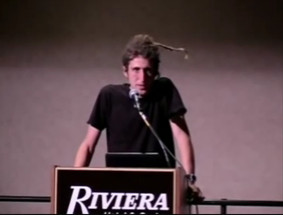
\includegraphics[scale=.7]{moxie}
    \caption{Moxie Marlinspike}
  \end{figure}
\end{frame}

\begin{frame}[fragile]{SSL X.509}
  \begin{itemize}
    \item SSL provides both confidentiality, integrity and identity
    \item CA signs a cert for a validated commonName: \emph{paypal.com}
    \item Client verifies server certificate commonName against requested domain
    \item X.509 is an ASN.1 based binary format
  \end{itemize}
  \begin{verbatim}
commonName ::=
  SEQUENCE{ { 2 5 4 3 }, StringType( SIZE(1..64) ) }
  \end{verbatim}
\end{frame}

\begin{frame}{X.509 ASN.1}
  \begin{itemize}
    \item IA5String defines a length-prefixed ASCII string
    \item Used for X.509 Certificate \texttt{commonName} field
  \end{itemize}
  \begin{figure}
    \begin{tabular}{*{20}{|c}}
      \hline
      $\backslash$x0E & w & w & w & . & p & a & y & p & a & l & . & c & o & m \\
      \hline 
    \end{tabular}
    \caption{ASN.1 IA5String}
  \end{figure}
\end{frame}

\begin{frame}{X.509 $\backslash0$ prefix attack}
  \begin{itemize}
    \item Common SSL libraries treat the commonName as a $\backslash0$-terminated C-string
    \item \texttt{strcmp()}
      \begin{itemize}
        \item \texttt{"www.paypal.com"}  
        \item \texttt{"www.paypal.com$\backslash0$.example.com"}
      \end{itemize} 
  \end{itemize}
  \begin{figure}
    \centering
    \Huge{PWNED!}
    \caption{You have been owned}
  \end{figure}
\end{frame}

\begin{frame}[fragile]{Conclusion}
  \begin{itemize}
    \item Common vulnerability across multiple independent implementations
    \begin{description}
      \item[Web Browsers] Firefox, IE, Chrome, Lynx, Curl
      \item[Mail Clients] Thunderbird, Outlook, Evolution
      \item[Chat Clients] Pidgin, AIM, irssi, centericq
      \item[SSL VPNs] AEP, Citrix, etc
    \end{description}
    \item Practical attack implemented in \textbf{sslstrip}
  \end{itemize}
\end{frame}

\end{document}
